\documentclass{article}
\usepackage{amssymb}
\usepackage[utf8]{inputenc}
\usepackage{amsmath}
\usepackage[spanish]{babel}
\usepackage{tikz}
\usepackage{graphicx}
\newcommand{\N}{\mathbb{N}}
\newcommand{\R}[1]{$\mathbb{R}^#1$}
\newcommand{\Phisub}[1]{$\varphi_#1$}
\newcommand{\matriz}[4]{\begin{pmatrix}
#1 & #2\\
#3 & #4
\end{pmatrix}}
\newcommand{\bx}{$\bar x \ $}
\newcommand{\bd}{$\bar d \ $}
\newcommand{\M}{M = \{x: Ax \leq b, x\geq 0\}}


\providecommand{\norm}[1]{\lVert#1\rVert}
\usepackage{amsthm}
\usepackage{graphicx}

\newtheorem{definition}{Definición}[section]
\newtheorem{observation}{Observación}[section]
\newtheorem{theorem}{Teorema}[section]
\newtheorem*{theorem*}{Teorema}
\newtheorem{proposition}{Proposición}[section]
\newtheorem{lemma}{Lema}[section]
\newtheorem{corollary}{Corolario}[section]
\newtheorem{example}{Ejemplo}[section]
\newtheorem{exercise}{Ejercicio}[section]



\title{	

	\normalfont\normalsize
	\textsc{Universidad de Murcia}\\ 
	\vspace{25pt} % Whitespace
	\rule{\linewidth}{0.5pt} % Thin top horizontal rule
	\vspace{20pt}\\ % Dará error hasta que escribas algo en el título
	{\huge Teoría Ol 2023
}\\ % The assignment title
	\vspace{12pt} % Whitespace
	\rule{\linewidth}{2pt}\\ % Thick bottom horizontal rule
	\vspace{12pt} % Whitespace
	% 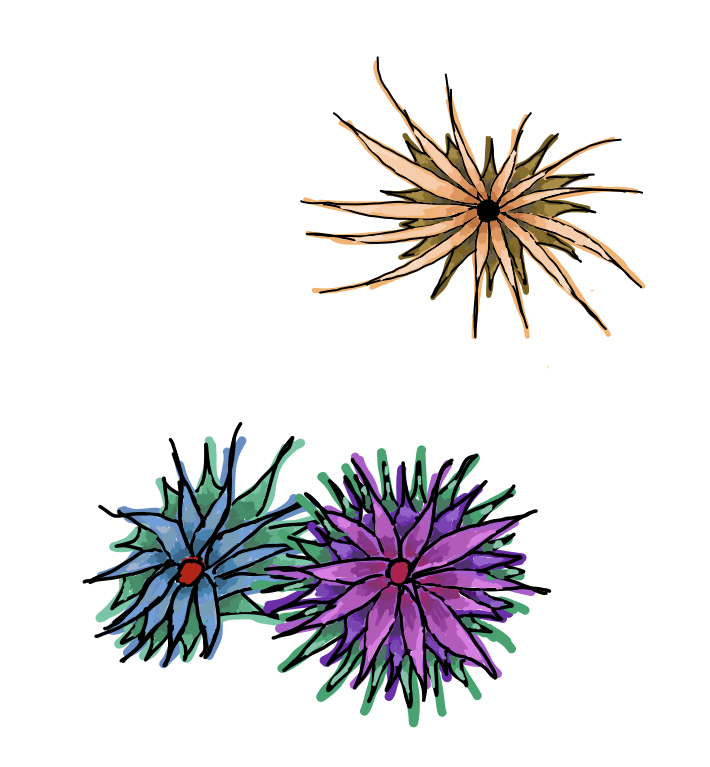
\includegraphics[scale=0.25]{floresportada.png}
}


\author{\LARGE Alonso Oma Alonso} % Your name

  
 
\date{\normalsize\today} % Today's date (\today) or a custom date



\begin{document}

\begin{titlepage}
	\maketitle
\end{titlepage}

\newpage
\tableofcontents
\newpage

\begin{section}{Teoría:}

	\begin{subsection}{Tema 3:}
		
        \begin{theorem*}{3.3}

            Sea $\bar x$ un punto de $M$. $\bar x$ es un punto extremo de $M$
            si se encuentra en $n$ hiperplanos definitorios linealmente indendientes.

            \begin{proof}
                \
                
                "$\Longleftarrow $" 
                
                $M = \{x: Ax \leq b, x\geq 0\}$
                \begin{itemize}
                    \item Supongamos \bx está en $n$ hiperplanos definitorios linealmente indendientes.
                    Sea $Gx = g$ el sistema definido por estos $n$ hiperplanos. Como $rg(G)=n$, el sistema es
                    \textbf{SCD}.
                    \item Por reducción al absurdo, supongamos que $x$ no es un punto extremo. $\bar x = \lambda x_1 + (1-\lambda)x_2$
                    con $x_1 \neq x_2 \in M, 0 < \lambda <1$.
                    \item En cada hiperplano donde \bx es conectante tambien lo son $x_1$ y $x_2$. Entonces $x_1$ y $x_2$ también son
                    soluciones de $Gx = g \Longrightarrow$ \textbf{CONTRADICCIÓN}
                \end{itemize}

                "$\Longrightarrow$"

                $M = \{x: Ax \leq b, x\geq 0\}$
                \begin{itemize}
                    \item Supongamos que \bx es punto extremos y es conectante a $h<n$ hiperplanos definitorios linealmente indendientes.
                    Sea $Gx=g$ el sistema definido por los hiperplanos en los que \bx es conectante. $rg(G) = h$.

                    \item El sistema $Gd = 0$ es \textbf{SCI}, pues $rg(G) = rg(G,0) = h < n$. Sea $\bar d \neq 0$ solución de $Gd = 0$.
                    \item $x_1 = \bar{x} + \epsilon \bar{d}, x_2 = \bar{x} - \epsilon \bar{d}$. $x_1$ y $x_2$ son conectantes en todos los hiperplanos
                    donde los es \bx (son soluciones del sistema $Gx = g$).

                    \item Considerenos una restricción $\alpha^t x \leq \beta$ en la que \bx no es conectante ($\alpha^t \bar{x} < \beta$).
                    \[\alpha^t x_1 = \alpha^t \bar{x} + \epsilon\alpha^t d<\beta +\epsilon \alpha^t d \quad\quad \alpha^t x_2 = \alpha^t \bar{x} - \epsilon\alpha^t d<\beta -\epsilon \alpha^t d\]

                    \item Es decir, para $\epsilon > 0$ suficientemente pequeño, $x_1$ y $x_2$ también satisfacen las otras restricciones en las que \bx no es conectante. Luego,
                    $x_!, x_2 \in M$ y $\bar{x} = \frac{1}{2}x_1 + \frac{1}{2}x_2$, lo cual es una contradicción.
                \end{itemize}
            \end{proof}
            
        \end{theorem*}

        \begin{theorem*}{3.5}
            
            Sea $\M$ un poliedro no vacío. Entonces el conjunto de puntos extremos es no vacío y tiene un número finito de puntos.

            \begin{proof}
                \

                $\M \neq \varnothing $. Sea $\bar{x} \in M$. Supongamos que \bx no es un punto extremo:
                \begin{itemize}
                    \item \bx está en $0\leq h <n$ hiperplanos definitorios linealmente indendientes.
                    \item $\bar{x} = \lambda x_1 + (1-\lambda)x_2$ con $x_1 \neq x_2 \in M, 0<\lambda < 1$.
                \end{itemize}
                Sea $d = x_2-x_1\neq 0 \rightarrow x_1=\bar{x}-(1-\lambda)d$ y $x_2 = \bar{x} + \lambda d$. En al menos uno de los sentidos
                $d$ o $-d$ no se puede avanzar indefinidamente a partir de $\bar{x}$, pues $M \subset \mathbb{R}^n$ (o el rayo toca en algún hiperplano
                $a^t_j x = b_j$ o en alguno de la forma $x_j = 0$). SIn perdida de generalidad, supongamos que eso ocurre en el sentido $-d$.

                Sea $\bar{\epsilon} = max\{\epsilon\geq 0: \bar{x}-\epsilon d \in M\}$ y sea $\bar{x}_1 = \bar{x} - \bar{e}d$. \bx está en el segmento dado por $\bar{x}_1$ y $\bar{x}_2$ lo que implica que $\bar{x}_1$ está en los hiperplanos definitorios en los que está \bx.
                Además, por construcción $\bar{x}_1$ está en alg´n otro hiperplano definitorio $\alpha^t x =\beta$.

                $\bar{x}_1$ está en $h+1$ hiperplanos linealmente indendientes. Si es punto extremo, \textbf{FIN}. En caso contrario, se repite el proceso.

                Supongamos que los $h$ hiperplanos en los que está \bx son $\{a^t_j x = b_j\}^h_{j=1}$ y supongamos que $\alpha^t x = \beta$ es combinación lineal de ellos $\longrightarrow \alpha = \sum_{j=1}^{h}\lambda_j a_j$. Entonces
                se tendría que $\alpha^t \bar{x}_1 = \beta = \sum_{j=1}^{h}\lambda_j a^t_j \bar{x}_1 = \sum_{j=1}^{h}\lambda_j b_j$. Por otro lado, $\alpha^t \bar{x} = \sum_{j=1}^{h}\lambda_j a^t_j \bar{x} = \sum_{j=1}^{h}\lambda_j b_j = \beta$.
                Es decir, si el nuevo hiperplano en el que $\bar{x}_1$ es conectante fuese linealmente dependiente de los anteriores, entonces \bx ya sería conectante sobre él, lo cuál es absurdo por construcción.
            \end{proof}
        \end{theorem*}

	\end{subsection}

\end{section}

\end{document}